\setcounter{exo}{0}

On s'intéresse au système de basculement de l'assise d'un système de fauteur roulant.
\begin{center}
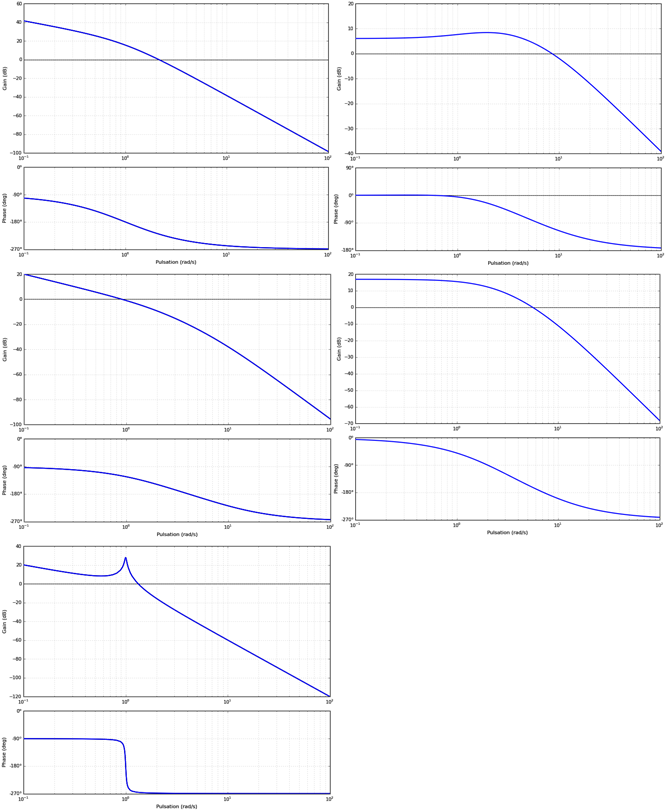
\includegraphics[width=\linewidth]{fig_01}
\end{center}

\begin{center}
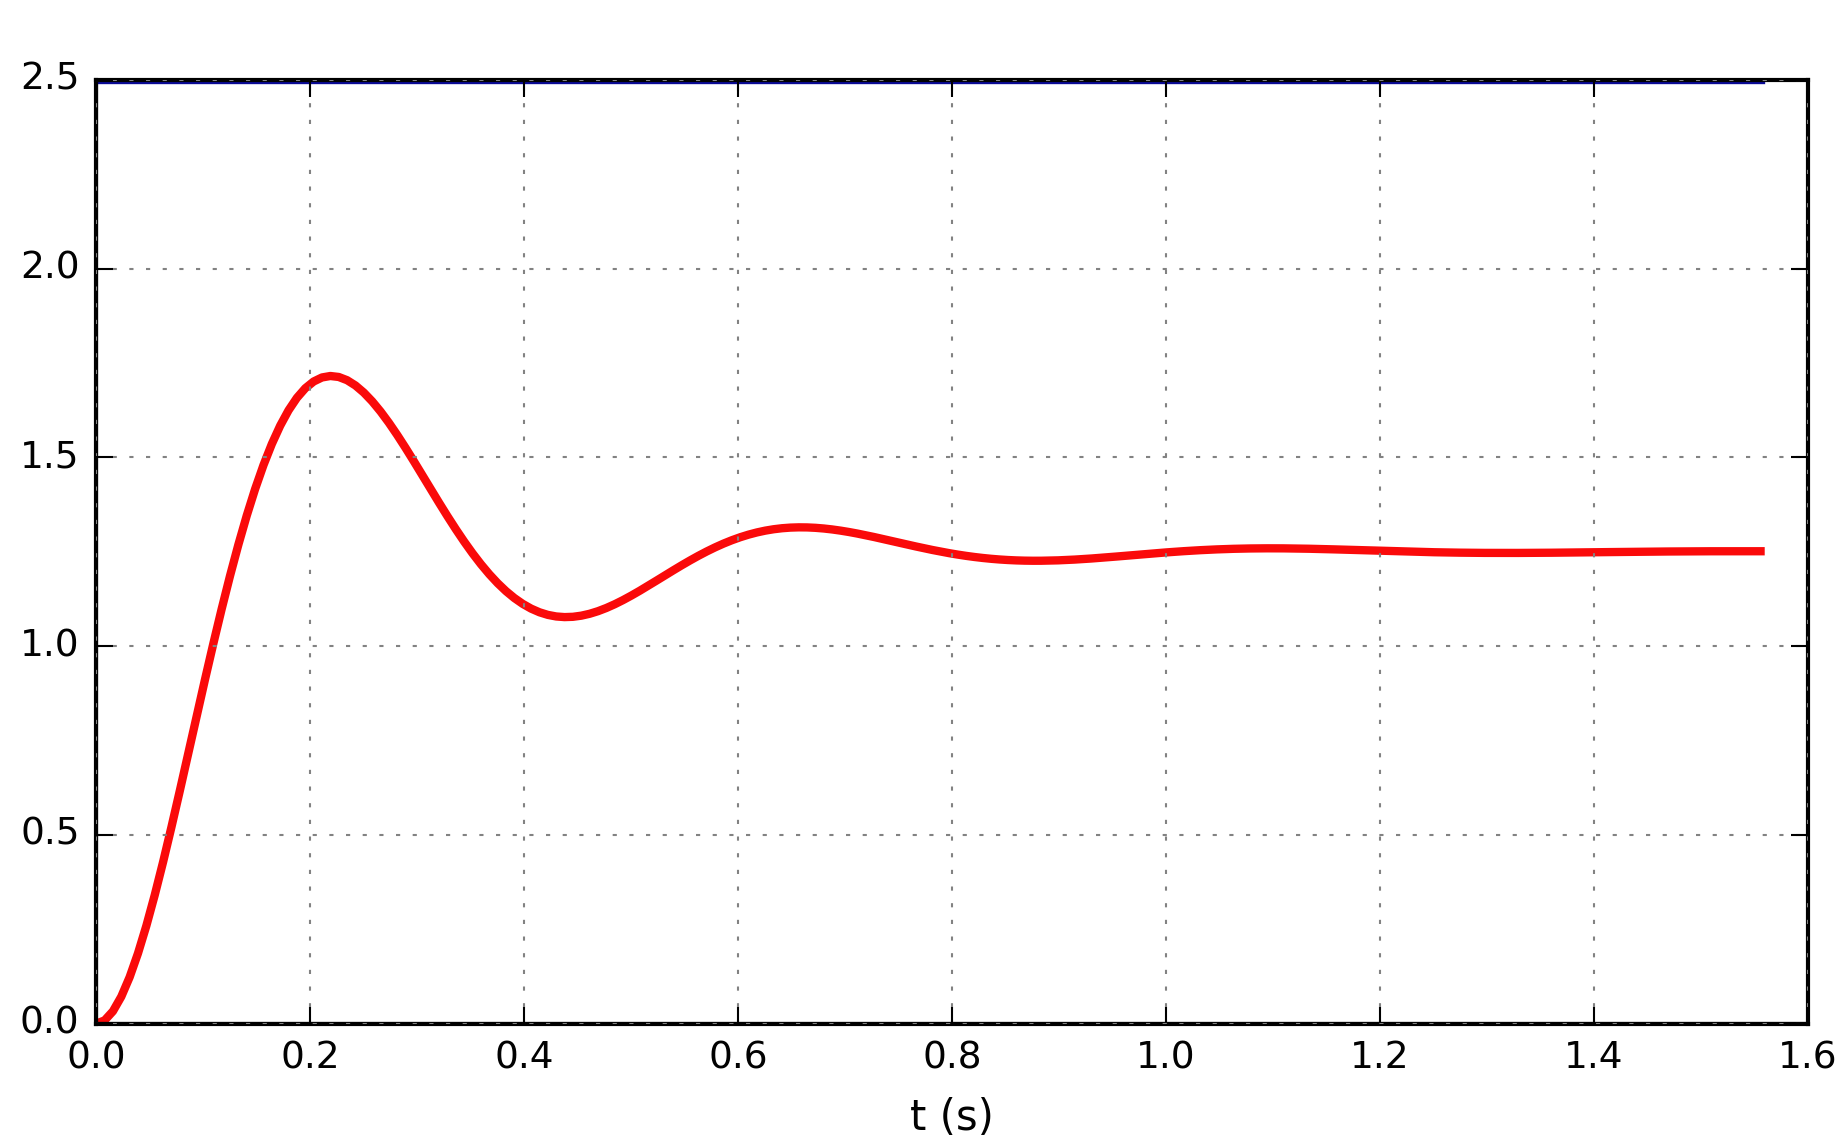
\includegraphics[width=.8\linewidth]{fig_02}
\end{center}

\subparagraph{}\textit{Déterminer les relations issues de la fermeture géométrique liant les paramètres $\gamma$, $\beta$ et $\lambda(t)$.}

\subparagraph{}\textit{En déduire l'expression de $\gamma$ en fonction de~$\beta$.}
